\documentclass[border=8pt]{standalone}
\usepackage[T1]{fontenc}
\usepackage{mathptmx}
\usepackage{tikz}
\usetikzlibrary{arrows.meta,positioning,fit,calc,shapes.geometric,shapes.misc,shapes.multipart,backgrounds}
\tikzset{
  arr/.style={-{Stealth[length=2.4mm,width=1.8mm]},line width=0.6pt},
  box/.style={draw,line width=0.6pt,align=center,rounded corners=2pt},
}

\begin{document}
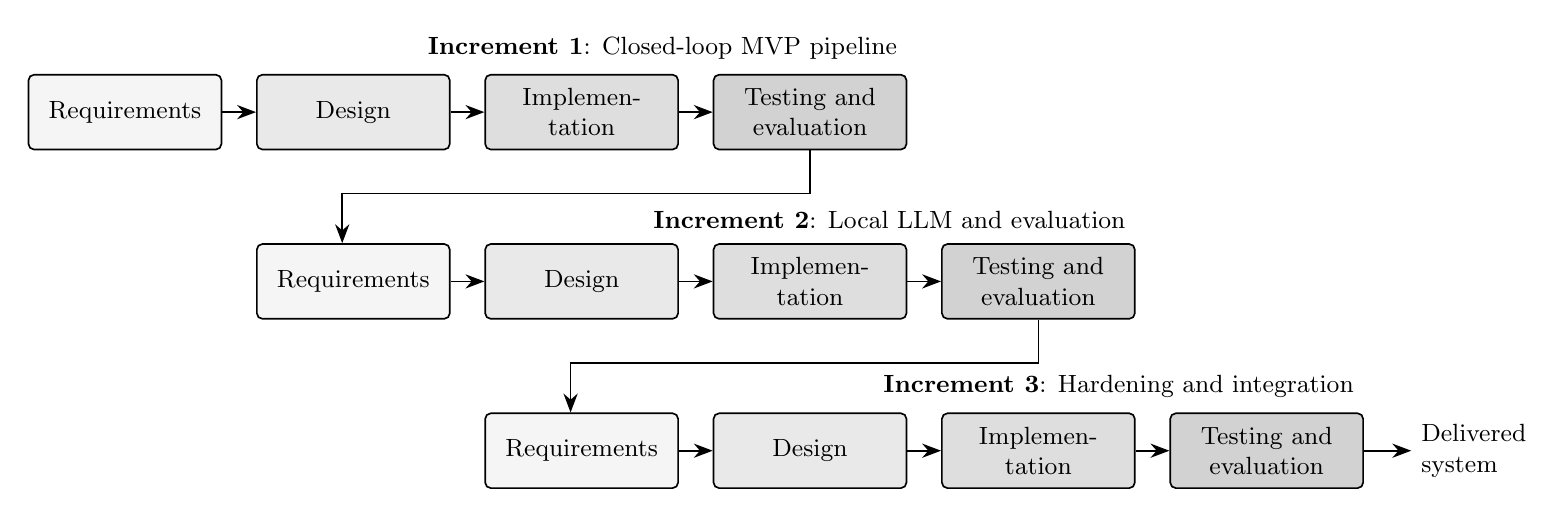
\begin{tikzpicture}[font=\small, p/.style={box, minimum width=2.45cm, minimum height=0.95cm}]
\node[anchor=south east] at (11.18,0.55) {\textbf{Increment 1}: Closed-loop MVP pipeline};
\node[p, fill=gray!8] (n11) at (1.25,0.00) {Requirements};
\node[p, fill=gray!17] (n12) at (4.15,0.00) {Design};
\node[p, fill=gray!26] (n13) at (7.05,0.00) {Implemen-\\tation};
\node[p, fill=gray!35] (n14) at (9.95,0.00) {Testing and\\ evaluation};
\draw[arr] (n11)--(n12);
\draw[arr] (n12)--(n13);
\draw[arr] (n13)--(n14);
\node[anchor=south east] at (14.08,-1.60) {\textbf{Increment 2}: Local LLM and evaluation};
\node[p, fill=gray!8] (n21) at (4.15,-2.15) {Requirements};
\node[p, fill=gray!17] (n22) at (7.05,-2.15) {Design};
\node[p, fill=gray!26] (n23) at (9.95,-2.15) {Implemen-\\tation};
\node[p, fill=gray!35] (n24) at (12.85,-2.15) {Testing and\\ evaluation};
\draw[arr] (n21)--(n22);
\draw[arr] (n22)--(n23);
\draw[arr] (n23)--(n24);
\node[anchor=south east] at (16.98,-3.75) {\textbf{Increment 3}: Hardening and integration};
\node[p, fill=gray!8] (n31) at (7.05,-4.30) {Requirements};
\node[p, fill=gray!17] (n32) at (9.95,-4.30) {Design};
\node[p, fill=gray!26] (n33) at (12.85,-4.30) {Implemen-\\tation};
\node[p, fill=gray!35] (n34) at (15.75,-4.30) {Testing and\\ evaluation};
\draw[arr] (n31)--(n32);
\draw[arr] (n32)--(n33);
\draw[arr] (n33)--(n34);
\draw[arr] (n14.south) -- ++(0,-0.55) -| ([xshift=-4pt]n21.north);
\draw[arr] (n24.south) -- ++(0,-0.55) -| ([xshift=-4pt]n31.north);
\draw[arr] (n34.east) -- ++(0.6,0) node[right, align=left] {Delivered\\ system};
\end{tikzpicture}
\end{document}